\Chapter{Approximations usuelles de l'équation du mouvement}
\label{ApproximationsEqMvt}
\begin{refsection}

La théorie fluide, en supposant une cohésion macroscopique de l'ensemble des
particules, fournit une description de base pour étudier les phénomènes de
transport dans les plasmas. A partir de ce formalisme, la plupart des modèles
sont construits en simplifiant les équations pour ne retenir que les
caractéristiques et processus essentiels du système à étudier. 

La première hypothèse communément retenue pour simplifier le modèle consiste à
considérer le tenseur de pression isotrope, ie.
$\boldsymbol{\Pi}_\alpha=0$, en supposant que les tranferts d'impulsion dus
aux collisions entre particules d'espèces différentes ont plus d'effet que
ceux résultants de la viscosité. L'équation du
mouvement~\eqref{1-eqMouvement} se réduit ainsi à un équilibre entre les forces
d'inertie, de traînée, de Lorentz et de pression :

\begin{equation}
\label{1-eqBilanForce}
\underbrace{m_\alpha n_\alpha\left(\partial_t \mathbf{u_\alpha} +
(\mathbf{u_\alpha}\cdot\nabla)\mathbf{u_\alpha}\right)}_\text{Inertie}
+\underbrace{m_\alpha n_\alpha\nu_\alpha\mathbf
u_\alpha}_\text{Traînée}=\underbrace{{q_\alpha n_\alpha}\left(\mathbf E+\mathbf
u_\alpha\times \mathbf B\right)}_\text{Forces électromagnétiques}
-\underbrace{{\nabla p_\alpha}}_\text{Pression}
\end{equation}
 
Le poids des différents termes de \eqref{1-eqBilanForce} varie en fonction des
paramètres du plasma et permet de définir le type d'écoulement des fluides
électroniques et ioniques. En mécanique des fluides, l'habitude est de définir
des nombres adimentionnés, dérivant des ratios entre les termes d'inertie, de
pression et de traînée, pour caractériser le fluide : ce sont les nombres de
Mach, de Reynolds et de Knudsen.

En physique des plasmas les fluides électroniques et ioniques sont couplés à
travers le champ électrique et le champ magnétique rend le transport très
anisotropique. Bien que l'on puisse dériver ici aussi des nombres
adimentionnés pour certains phénomènes tels que la transition
subsonique-supersonique, la catégorisation des écoulements est plus compliquée
et l'on préfère simplifier davantage l'expression de la vitesse fluide.

Dans le domaine des plasmas de fusions fortement magnétisés, il est d'usage de
considérer le petit paramètre $\delta=\rho_L/L$ pour moyenner l'équation
\eqref{1-eqBilanForce} sur les échelles rapides. Dans le domaine des plasmas
froid, on fait plutôt l'hypothèse de forte collisionnalité et on développe
l'équation du mouvement en fonction du petit paramètre $\lambda_{lpm}/L$.

Un premier cas limite peut être obtenu quand le terme de pression domine
sur l'ensemble des termes du membre de gauche de \eqref{1-eqBilanForce}, qui en
les négligeant, se transforme en :

\begin{equation}
\label{1-equilibreBoltzman}
q_\alpha\mathbf
E =\frac{e}{n_\alpha}\nabla n_\alpha T_\alpha
\end{equation}

C'est la relation de Boltzmann. Ce cas de figure est caractéristique pour les
électrons non-collisionnels enfermés dans un puit de potentiel (par exemple résultant de
l'interaction entre le plasma et les parois). En l'absence de champ magnétique
ou parallèlement aux lignes de champ, le champ électrique et le gradient de
pression se compensent, amenant les électrons dans un équilibre de Boltzmann,
ie. où les particules suivent une distribution de Boltzmann :

\begin{equation}
\label{1-profilBoltzman}
n_\alpha=n_0\exp(q_\alpha \Phi/eT_\alpha)
\end{equation}

Cette hypothèse est fondamentale dans la dérivation des modèles fluides de
transport pour les plasmas dans la mesure où elle constitue l'une des bases de
la théorie des gaines vue précédement. 

\section{Approche par les vitesses de dérive}
\label{vitessesDerive}
L'approche par les vitesses de dérive est à la base de nombreux modèles
développés pour étudier le transport dans les plasmas de fusion par
confinement magnétique~\parencite{Garcia,Bisai,Tamain}. Dans cette approche, la
vitesse des particules est exprimée en fonction du mouvement cyclotronique rapide, d'une composante
parallèle au champ magnétique et d'une dérive lente du centre-guide des particules dans
la direction transverse. Cette décomposition, qui peut se voir comme une
version fluide de la théorie particulaire du centre-guide, sous-entend que les
fréquences cyclotroniques sont grandes devant les fréquences caractéristiques du
transport, ie. $\omega_{ce},\omega_{ci}\gg\omega$. 
 
\subsection{Les plasmas de la Scrape-off-Layer}
La Scrape-Off-Layer des tokamaks, ou SOL, est la zone en
périphérie du plasma confiné, ie. qui commence à partir de la séparatrice et qui
peut éventuellement s'étendre jusqu'aux parois internes du tore (voir
figure~\ref{SOL}). Dans cette région, les
particules ne sont plus confinées car les lignes de champ interceptent un
obstacle matériel (un limiteur ou un divertor) traité et dessiné spécifiquement
pour supporter les flux de matière et de chaleur qui s'échappent du plasma de
c\oe ur par transport transverse.
En conséquence, les profils de densité et de température s'effondrent sur une
longueur caractéristique qui définit la largeur de la SOL, $\lambda_\text{SOL}$,
donnant naissance à de forts gradients qui maintiennent le plasma hors
de l'équilibre thermodynamique.

\begin{figure}[!htbp]
    \centering
	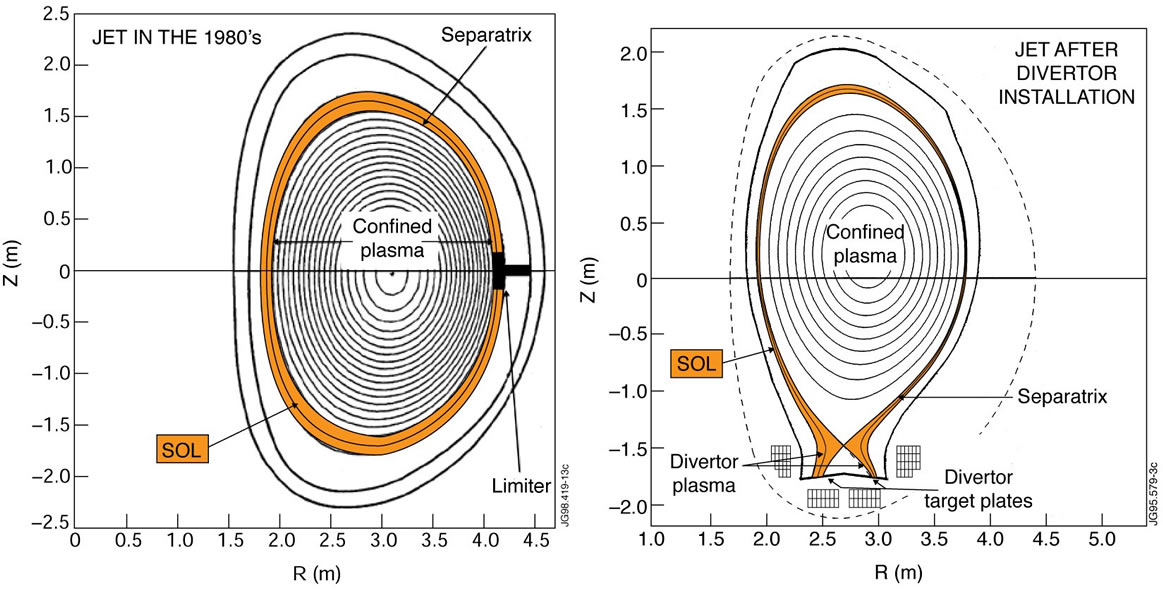
\includegraphics[height=80mm]{figures/1-limiterDivertor.jpg}
	\caption{Section verticale du tokamak JET en version limiteur
	(à gauche) et divertor (à droite). La SOL est illustrée en
	orange~\parencite{efda}.}\label{SOL}
\end{figure}
 
Typiquement, les plasmas de SOL ont une densité de
l'ordre de 10$^{19}$~m$^{-3}$ et une température inférieure à la centaine
d'électronvolts. A cette température, le plasma est presque totalement ionisé et
le champ magnétique, d'environ 3T, confine efficacement les particules dans un
mouvement cyclotronique de fréquence $\omega_{ci}\sim45$~MHz pour un proton et
$\omega_{ce}\sim80$~GHz pour un électron, toutes deux bien supérieures à la
fréquence caractéristique du transport parallèle :

\begin{equation}
\omega_\para\sim
\frac{v_{\text{T}\alpha}}{L_\para}\approx\omega_{c\alpha}\frac{\rho_{L\alpha}}{L_\para}\rightarrow
\delta=\frac{\omega_\para}{\omega_{c\alpha}}\ll1
\end{equation} 

Dans la direction perpendiculaire au champ
magnétique, les vitesses de dérive associées aux gradients transverses (dont les longueurs
typiques $L_\nabla$ de quelques centimètres sont bien supérieures aux rayon de
Larmor ionique $\rho_{Li}\approx3.10^{-4}$~m et électroniques
$\rho_{Le}\approx7.10^{-6}$~m) entraînent un transport de fréquence
caractéristique $\omega_\perp\sim v_\perp/L_\para\sim\rho_{L\alpha}
v_{\text{T}\alpha}/(L_\para L_\nabla)$ de deux ordres de grandeur inférieur à
$\omega_{c\alpha}$ :

\begin{equation}
\frac{\omega_\perp}{\omega_{c\alpha}}\approx\frac{\rho_{L\alpha}^2}{L_\para
L_\nabla}=\delta^2
\end{equation}

Malgré leur faible fréquence, ces vitesses de dérives sont à l'origine de tous
les mécanismes de micro-turbulence et jouent ainsi un rôle primordiale dans le
problème du confinement des plasmas de fusion.

\subsection{Vitesses de dérive électrique et diamagnétique}

Quand le degré d'ionisation du plasma est très élevé, le terme issu de
l'interaction avec le gaz peut être négligé dans l'équation du
mouvement~\eqref{1-eqBilanForce} :

\begin{equation}
\label{1-eqSOL}
 m_\alpha n_\alpha\left(\partial_t \mathbf{u_\alpha} +
(\mathbf{u_\alpha}\cdot\nabla)\mathbf{u_\alpha}\right)
={q_\alpha n_\alpha}\left(\mathbf E+\mathbf
u_\alpha\times \mathbf B\right)
-{\nabla p_\alpha}
\end{equation}

 Sous l'hypothèse de faible variation spatiale des grandeurs et des champs à
 l'échelle du rayon de Larmor, la lente évolution du système par rapport aux
 fréquences cyclotroniques permet d'effectuer un développement de l'équation du
 mouvement en fonction du petit paramètre $\delta$. En négligeant le
 mouvement cyclotronique, qui correspond à l'ordre 0 de ce développement et qui
 est de moyenne nulle sur un temp $t\sim\omega_{c\alpha}^{-1}$, la projection
 de~\eqref{1-eqSOL} perpendiculairement au champ magnétique s'écrit à l'ordre 1
 en $\delta$ :
 
 \begin{equation}
\label{1-eqSOLperp}
0
={q_\alpha n_\alpha}\left(\mathbf E+\mathbf
u_{\alpha\perp}^{(1)}\times \mathbf B\right)
-{\nabla_\perp p_\alpha}
\end{equation}

En prenant le produit vectoriel par $\mathbf B$ de cette équation, on obtient
les deux vitesses de dérive fluides principales, la vitesse de dérive électrique
$\mathbf u_E$ et la vitesse de dérive diamagnétique $\mathbf u_*$, relativement
liées aux gradients transverses de potentiel électrique $\Phi$ et de pression
$p_\alpha$:

\begin{equation}
\mathbf u_{\alpha\perp}^{(1)}=\mathbf u_E+\mathbf u_*=\frac{\mathbf
B\times\nabla_\perp \Phi}{B^2}-\frac{\mathbf B\times\nabla_\perp
p_\alpha}{n_\alpha q_\alpha B^2}
\end{equation}

L'origine de ces vitesses de dérive est illustrée sur la
figure~\ref{1-vitessesDerive}. La dérive diamagnétique est une vitesse
purement fluide qui traduit le mouvement d'ensemble des particules, et non
une dérive individuelle de celles-ci. De ce fait, elle ne transporte que
très peu de matière en comparaison de la dérive électrique : pour s'en
convaincre, il suffit de regarder la divergence des flux issus de ces
vitesses :

\begin{equation}
\nabla\cdot\left(n_\alpha\mathbf
u_E\right)=\nabla\cdot\left(n_\alpha\frac{\mathbf B\times\nabla
\Phi}{B^2}\right) =\nabla\frac{n_\alpha}{B}\times\nabla \Phi\cdot \mathbf b
\end{equation}

\begin{equation}
\nabla\cdot\left(n_\alpha\mathbf
u_*\right)=\nabla\cdot\left(\frac{\mathbf B\times\nabla
p_\alpha}{q_\alpha B^2}\right)
=\frac{1}{q_\alpha}\nabla p_\alpha\times\nabla\frac{1}{B}\cdot \mathbf b
\end{equation}

La divergence du flux diamagnétique est donc nulle aux effets de courbure du
champ magnétique près. Par contre, et comme
précisé au paragraphe \S\ref{1-plasma-champMag}, la dérive diamagnétique est 
sensible à la charge des particules et est donc la seule à porter du courant.
L'influence de ce courant est fondamental dans la stabilité du plasma :

\begin{equation}
\mathbf j_*=e(n_i\mathbf u^i_*-n_e\mathbf
u^e_*)=e(\nabla(p_i+p_e)\times\mathbf B/B^2)
\end{equation}

\begin{figure}[!htbp]
    \centering
	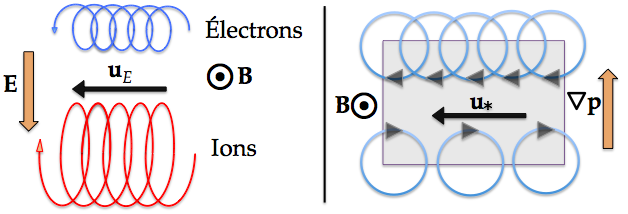
\includegraphics[height=80mm]{figures/1-vitessesDerive.jpg}
	\caption{Interprétation des vitesses de dérive électrique et diamagnétique.}
	\label{1-vitessesDerive}
\end{figure}


\subsection{Dérive de polarisation}

Dans le cas d'un champ électrique variant lentement dans le temps, une troisième
dérive, d'un ordre de grandeur inférieur aux dérives électrique et diamagnétique,
peut être identifiée : 

\begin{equation}
\label{1-vitessePol}
\mathbf{u}_\perp^{(2)}= \text{d}\mathbf
u_\perp^{(1)}/\text{dt}=\text{d}(\mathbf
u_E+\mathbf
u_*)/\text{dt}
\end{equation}

Par un calcul compliqué, on peut montrer que la dérivée totale de la dérive
diamagnétique est exactement compensée par la prise en compte du tenseur des
contraintes de Braginskii (les termes non-diagonaux du tenseur de
pression). L'expression de cette dérive d'ordre 2 se réduit alors à :

\begin{equation}
\label{1-vitessePol}
\mathbf{u}_\perp^{(2)}= \frac{\text{d}\mathbf
u_E}{\text{dt}}=-\frac{m_\alpha}{q_\alpha B^2}\frac{\text{d}\nabla_\perp
\Phi}{\text{dt}}
\end{equation}

C'est la dérive de polarisation $\mathbf{u}_\perp^{(2)}=\mathbf u^\alpha_p$, qui
dérive du terme d'inertie. Bien qu'elle soit d'un ordre de grandeur inférieur aux deux autres
vitesses de dérive, la divergence du flux qui lui est associé est comparable à celle du
flux diamagnétique. Comme la dérive électrique n'a aucune influence sur
l'évolution du courant, la contribution de la dérive de polarisation est dès
lors du même ordre de grandeur que celle de la dérive diamagnétique et ne peut plus
être négligée.

\section{Equation de dérive-diffusion}
\label{1-transportAmbipolaire}
\subsection{Equation de dérive-diffusion non magnétisée}
Les plasmas froids de décharge utilisés dans l'industrie et la recherche n'ont
en général qu'un faible degré d'ionisation $\alpha<$1\% et la dynamique des
espèces y est dominée par la perte de quantité de mouvement liée à l'ionisation
et aux collisions avec le gaz. Pour modéliser ce type de plasma, la prise en
compte du terme collisionnel dans l'équation du mouvement est essentielle.
En l'absence de champ magnétique, le rapport d'échelle entre le libre parcours moyen des particules
et la taille du plasma $\lambda_\alpha\ll L$ permet de simplifier l'équation du
mouvement en négligeant les termes d'inertie, relativement faibles\footnote{Les
termes inertiels peuvent être négligés quand la vitesse fluide $\mathbf u$ est
subsonique : $\mathbf u$ vérifie alors $\mathbf u\ll \left<v\right>/K_n$, où
$K_n=\lambda/L$ est le nombre de Knudsen et $$\nu \mathbf u=\frac{
\left<v\right>\mathbf u}{\lambda}\gg \frac{u^2}{\lambda}K_n=\frac{u^2}{L}\sim
\mathbf u\cdot\nabla\mathbf u$$} par rapport au terme collisionnel :

\begin{equation}
\label{1-eqDriftDif}
n_\alpha\mathbf u_\alpha=\frac{q_\alpha}{\nu_\alpha m_\alpha}n_\alpha\mathbf
E-\frac{\nabla\left(n_\alpha eT_\alpha\right)}{\nu_\alpha
m_\alpha}\equiv\frac{q_\alpha}{|q_\alpha|}\mu_\alpha n_\alpha\mathbf
E-{\nabla\left(D_\alpha n_\alpha\right)}
\end{equation}

C'est l'équation de dérive-diffusion, avec les coefficients de
transport $\mu_\alpha$ et $D_\alpha$, tous deux
inversement proportionnels à la fréquence de collision $\nu_\alpha$ (donc à la
densité de gaz), et reliés par la relation d'Einstein :

\begin{equation}
\label{1-EinsteinRelation}
D_\alpha/\mu_\alpha=T_\alpha
\end{equation}

\begin{itemize}
  \item la mobilité, définie par $\mu_\alpha=q_\alpha/\nu_\alpha m_\alpha$,
  mesure la disposition d'une espèce à laisser passer le courant au sein d'un milieu
  \item la diffusion, de coefficient $D_\alpha=eT_\alpha/\nu_\alpha m_\alpha$,
  représente la tendance naturelle d'un système à rendre homogène sa densité de particule sous l'effet
  de l'agitation thermique.
\end{itemize}

En combinant \eqref{1-eqDriftDif} avec l'équation de continuité
\eqref{1-eqContinuite}, on obtient une équation d'évolution de la densité
constituée d'une loi d'Ohm et d'une loi de Fick :
 
\begin{equation}
\label{1-eqDriftDifContinuite}
\partial_t
n_\alpha=\nabla\cdot(\underbrace{\frac{q_\alpha}{|q_\alpha|}\mu_\alpha n_\alpha\mathbf E}_\text{Loi d'Ohm}+\underbrace{D_\alpha{\nabla n_\alpha}}_\text{Loi
de Fick})+S_\alpha
\end{equation}

Dans des plasmas de décharge collisionnels, à partir de la source d'ionisation,
les électrons ont tendance à se déplacer beaucoup plus rapidement que les ions
du fait de leur faible masse et de leur température. Cette différence de
mobilité entraîne l'apparition d'un champ électrique dit "ambipolaire"
$\mathbf E_a$, faisant dériver les ions et les électrons ensembles et
systématiquement dirigé dans le sens opposé du gradient de densité afin de
limiter la diffusion des électrons et accélérer les ions. En ne considérant
qu'une seule espèce ionique, on trouve son expression en cherchant le champ
correspondant à un courant nul :
 
\begin{equation}
\label{1-eqEAmb}
\mathbf j=0 \Rightarrow \mathbf E=\mathbf
E_a=\frac{D_i-D_e}{\mu_i+\mu_e}\frac{\nabla n}{n}
\end{equation}

A l'interface entre les parois et le plasma, une gaine positive se
forme et enferme les électrons dans un puit de potentiel. Ce phénomène, en plus
des collisions, permet une isotropisation rapide de la fonction de distribution
des électrons, qui peuvent alors être considérés en équilibre de Boltzmann.
Les ions, quant-à-eux, ont une durée de vie de l'ordre de
$\nu_\text{iz}\puissance{-1}$ : depuis leur zone de création, ils sont
continuement accélérés par le champ ambipolaire jusqu'à être perdus à la paroi
où ils se recombinent. La théorie classique des gaines prédit qu'à l'équilibre,
la densité diminue d'un facteur 2 et la chute de potentiel ambipolaire est
de l'ordre de $T_e/2$ (cf. \S\ref{1-gaines}.

\subsection{Equation de dérive-diffusion magnétisée}
\label{1-deriveDiffMag}
L'utilisation d'un champ magnétique dans un plasma permet de contrôler en partie
le transport des particules et d'obtenir des configurations favorables pour
diverses applications. Cependant, la prise en compte du terme de Laplace dans
\eqref{1-eqBilanForce} impose une forte anisotopie dans le système, ce qui
complexifie considérablement les phénomènes de transport : en
négligeant l'inertie, on peut considérer \eqref{1-eqBilanForce} comme une
équation algébrique d'inconnue $\mathbf u$ qui s'écrit sous une forme
tensorielle de l'équation de dérive-diffusion :

\begin{equation}
\label{1-eqDriftDif}
n_\alpha\mathbf u_\alpha=\frac{q_\alpha}{|q_\alpha|}\mu_\alpha
n_\alpha\left(\mathbf E+\mathbf u_\alpha\times\mathbf
B\right)-\nabla\left(D_\alpha n_\alpha\right)\equiv
\frac{q_\alpha}{|q_\alpha|} n_\alpha\boldsymbol{\mu}_\alpha\cdot \mathbf
E-{\nabla\left(\mathbf{D}_\alpha n_\alpha\right)}
\end{equation}

où la mobilité $\boldsymbol{\mu}_\alpha$ et la diffusion $\mathbf{D}_\alpha$
sont devenus des tenseurs d'ordre 2 :

\begin{align}
\boldsymbol{\mu}_\alpha =
 \begin{pmatrix}
  \mu_{\alpha\perp} & \mu_{\alpha\times} & 0 \\
  \mu_{\alpha\times} & \mu_{\alpha\perp} & 0 \\
  0  & 0  & \mu_{\alpha\para} 
 \end{pmatrix}\;\;\;\;\text{et}\;\;\;\;
 \mathbf D_\alpha =
 \begin{pmatrix}
  D_{\alpha\perp} & D_{\alpha\times} & 0 \\
  D_{\alpha\times} & D_{\alpha\perp} & 0 \\
  0  & 0  & D_{\alpha\para} 
 \end{pmatrix}
\end{align}

Dans la direction parallèle au champ magnétique, les coefficients de mobilité et
de diffusion sont inchangés
$\mu_{\alpha\para}=\mu_{\alpha}=q_\alpha/m_\alpha\nu_\alpha$ et
$D_{\alpha\para}=D_\alpha=eT_\alpha/m_\alpha\nu_\alpha$. Les coefficients de la
direction perpendiculaire font quant à eux apparaître le paramètre de Hall
$h_\alpha=\omega_{c\alpha}/\nu_\alpha$ :

\begin{align}
\mu_{\alpha\perp}=\frac{1}{1+h_\alpha^2}\mu_\alpha\;\;\;\;\;\;\;\;
\;\;\;\;D_{\alpha\perp}=\frac{1}{1+h_\alpha^2}D_\alpha
\end{align}
\begin{align}
\mu_{\alpha\times}=\frac{h_\alpha}{1+h_\alpha^2}\mu_\alpha\;\;\;\;
\;\;\;\;\;\;\;\;D_{\alpha\times}=\frac{h_\alpha}{1+h_\alpha^2}D_\alpha
\end{align}

Quand $h_\alpha=0$, les tenseurs sont diagonaux et isotropes. Ensuite, plus le
facteur de hall augmente, plus le transport dans les directions transverses se
réduit :
les coefficients indicés avec le symbole perpendiculaire sont inversement
proportionnels au carré du champ magnétique $\mu_{\alpha\perp},
D_{\alpha\perp}\propto B\puissance{-2}$ ; à partir de $h_\alpha=1$, le
transport croisé commence à dominer sur le transport collisionnel et devient proportionnel à
$B\puissance{-1}$. Cette loi de puissance que suit le transport par rapport au
champ magnétique est souvent interprétée comme la signature d'un transport
anormal, mais apparaît naturellement dans les équations à travers les
coefficients $\mu_{\alpha\times}$ et $D_{\alpha\times}$.



%\bibliographystyle{apalike}
%\bibliography{biblio}
\end{refsection}

